\documentclass[	DIV=calc,%
							paper=a4,%
							fontsize=12pt,%
							twocolumn]{scrartcl}	 					% KOMA-article class

\usepackage{lipsum}													% Package to create dummy text
\usepackage[english]{babel}										% English language/hyphenation
\usepackage[protrusion=true,expansion=true]{microtype}				% Better typography
\usepackage{amsmath,amsfonts,amsthm}					% Math packages
\usepackage[pdftex]{graphicx}									% Enable pdflatex
\usepackage[svgnames]{xcolor}									% Enabling colors by their 'svgnames'
\usepackage[hang, small,labelfont=bf,up,textfont=it,up]{caption}	% Custom captions under/above floats
\usepackage{epstopdf}												% Converts .eps to .pdf
\usepackage{subfig}													% Subfigures
\usepackage{booktabs}												% Nicer tables
\usepackage{fix-cm}													% Custom fontsizes
\usepackage{natbib}                                                 % Bibliography
\setcitestyle{authoryear,open={(},close={)}}            %Citation-related commands
\usepackage{hyperref}
\hypersetup{
    colorlinks=true,
    linkcolor=blue,
    filecolor=blue,      
    urlcolor=blue,
    citecolor = blue,
    pdftitle={RTU DESS Format},
    pdfpagemode=FullScreen,
    }
\usepackage{float}

%%% Custom sectioning (sectsty package)
\usepackage{sectsty}													% Custom sectioning (see below)
\allsectionsfont{%															% Change font of al section commands
	\usefont{OT1}{phv}{b}{n}%										% bch-b-n: CharterBT-Bold font
	}

\sectionfont{%																% Change font of \section command
	\usefont{OT1}{phv}{b}{n}%										% bch-b-n: CharterBT-Bold font
	}



%%% Headers and footers
\usepackage{fancyhdr}												% Needed to define custom headers/footers
	\pagestyle{fancy}														% Enabling the custom headers/footers
\usepackage{lastpage}	

% Header (empty)
\lhead{}
\chead{}
\rhead{}
% Footer (you may change this to your own needs)
\lfoot{\small \usefont{OT1}{lmr}{c}{n} \textcolor{blue}{Short Research Title}}
\cfoot{}
\rfoot{\footnotesize page \thepage\ of \pageref{LastPage}}	% "Page 1 of 2"
\renewcommand{\headrulewidth}{0.0pt}
\renewcommand{\footrulewidth}{0.4pt}

\usepackage[font=small,format=plain,labelfont=bf,
textfont=normal,singlelinecheck=false]{caption}

%%% Creating an initial of the very first character of the content
\usepackage{lettrine}
\newcommand{\initial}[1]{%
     \lettrine[lines=3,lhang=0.3,nindent=0em]{
     				\color{DarkBlue}
     				{\textsf{#1}}}{}}



%%% Title, author and date metadata
\usepackage{titling}															% For custom titles

\newcommand{\HorRule}{\color{Black}%			% Creating a horizontal rule
									  	\rule{\linewidth}{2pt}%
										}
%%begin novalidate
\pretitle{\vspace{-60pt} \begin{flushleft} \HorRule 
				\fontsize{50}{50} \usefont{OT1}{phv}{b}{n} \color{DarkBlue} \selectfont 
				}
\title{Research Title}					% Title of your article goes here
\posttitle{\par\end{flushleft}\vskip 0.5em}

\preauthor{\begin{flushleft}
					\fontsize{20}{50} \lineskip 0.5em \usefont{OT1}{lmr}{b}{ol} \color{DarkRed}}
\author{Lee Dong Min$^{1, 2,\star}$, Kim Moon Bin$^{1,3}$, Yoon Sanha$^{1,4}$, \newline Kim Myung Jun$^{1,5}$, : Park Jin Woo$^{1,6}$, and Park Min Hyuk$^{1,7}$ }											% Author name goes here
\postauthor{\fontsize{15}{10} \usefont{OT1}{lmss}{bx}{ol} \newline \newline \color{Black} 
								$^{1}$Mercury
        \newline                $^{2}$Venus
        \newline                $^{3}$Earth
        \newline                $^{4}$Mars
        \newline                $^{5}$Jupiter
        \newline                $^{6}$Saturn
        \newline                $^{7}$Neptune
					\par\end{flushleft}\HorRule
     
     \fontsize{10}{50} \usefont{OT1}{pmt}{b}{n} \color{black}
    $^\star$Corresponding Author: leedongmin@astro.aroha.com}
%%end novalidate
\date{}																% No date



%%% Begin document
\begin{document}
\maketitle
\thispagestyle{fancy} 			% Enabling the custom headers/footers for the first page 
% The first character should be within \initial{}
\section*{Abstract}
\initial{\textbf{T}}\textbf{his is where you will insert your abstract. Brief summary, important points, interesting results/developments, methods developed/used, research gap being resolved, and outline of the paper must be included in the abstract. Make sure that there is no reference/cited article in your abstract. No more than 250 words should be in this part.}

\section*{Introduction}
\; \; %% '\; \;' is required for indention
\lipsum[20] \citep{Ref1}. %use \citet{} for "Kuo et al. (2022)"

\lipsum[5]

\lipsum[5]

\section*{Methodology}
\; \; %% '\; \;' is required for indention
\lipsum[6]
\begin{itemize}
	\item \lipsum[7] 
	\item \lipsum[7] 
	\item \lipsum[7] 
\end{itemize}

\lipsum[6]

\section*{Results}
\; \; %% '\; \;' is required for indention
\lipsum[7] (see Table~\ref{Tab1}) 

\subsection*{Result 1}
\; \; %% '\; \;' is required for indention 
\lipsum[7] (see Figure~\ref{Figure 1})

\begin{table}
\caption{Caption of table}
\centering
	\begin{tabular}{llr}
		\toprule
		\multicolumn{2}{c}{Name} \\
		\cmidrule(r){1-2}
			First name & Last Name & Grade \\
		\midrule
			John & Doe & $7.5$ \\
			Richard & Miles & $2$ \\
		\bottomrule
	\end{tabular}
 \label{Tab1}
\end{table}


\begin{figure}[H]
    \centering
    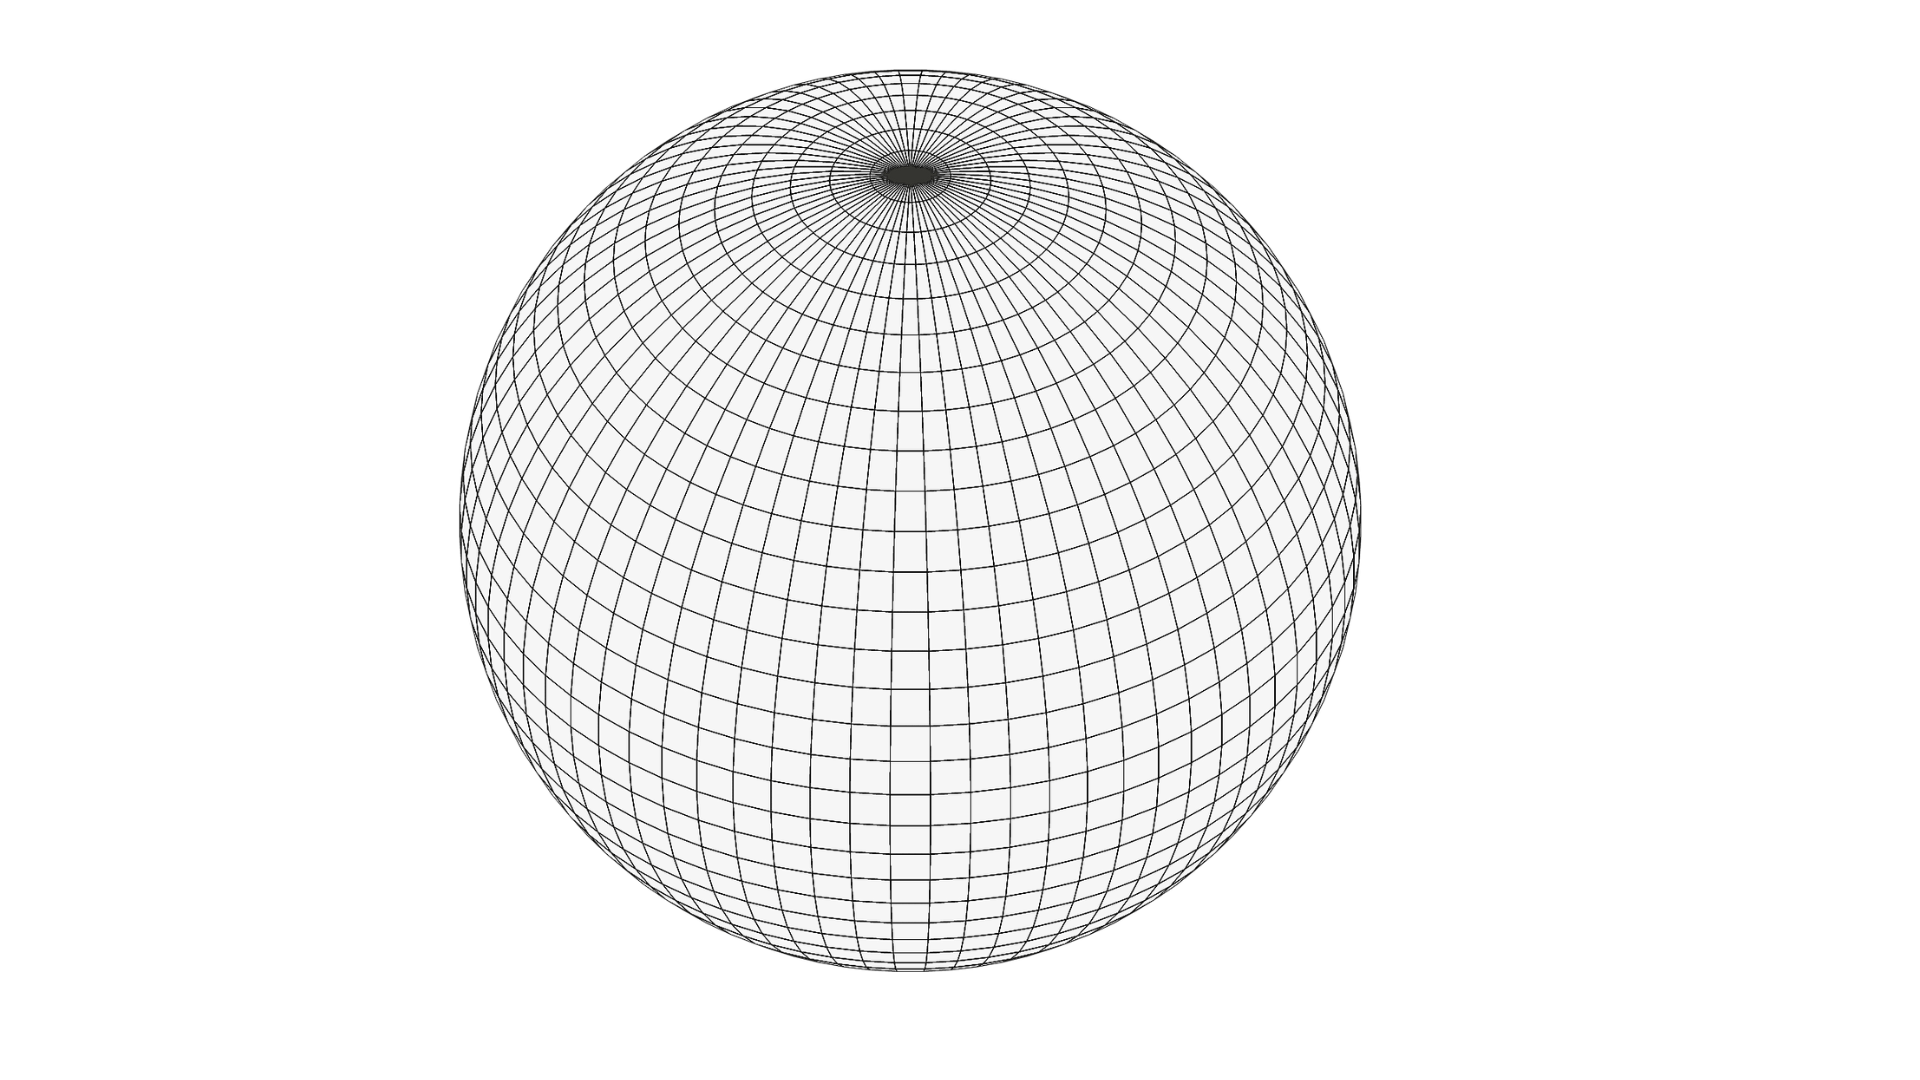
\includegraphics[width=\columnwidth]{7.png}
    \caption{Sphere Mesh}
    \label{Figure 1}
\end{figure}

\section*{Discussion}
\; \; %% '\; \;' is required for indention
\lipsum[7]

\begin{description}
	\item[First] \lipsum[30] 
	\item[Last] \lipsum[30] 
\end{description}

\lipsum[3] 
According to \citet{Ref1} and \citet{Ref2}, %For multiple citations use ',' in between references
\lipsum[2] 

\begin{figure}[H] %'[H]' forces the figure to stay in the relative position of the text it is located
    \centering
    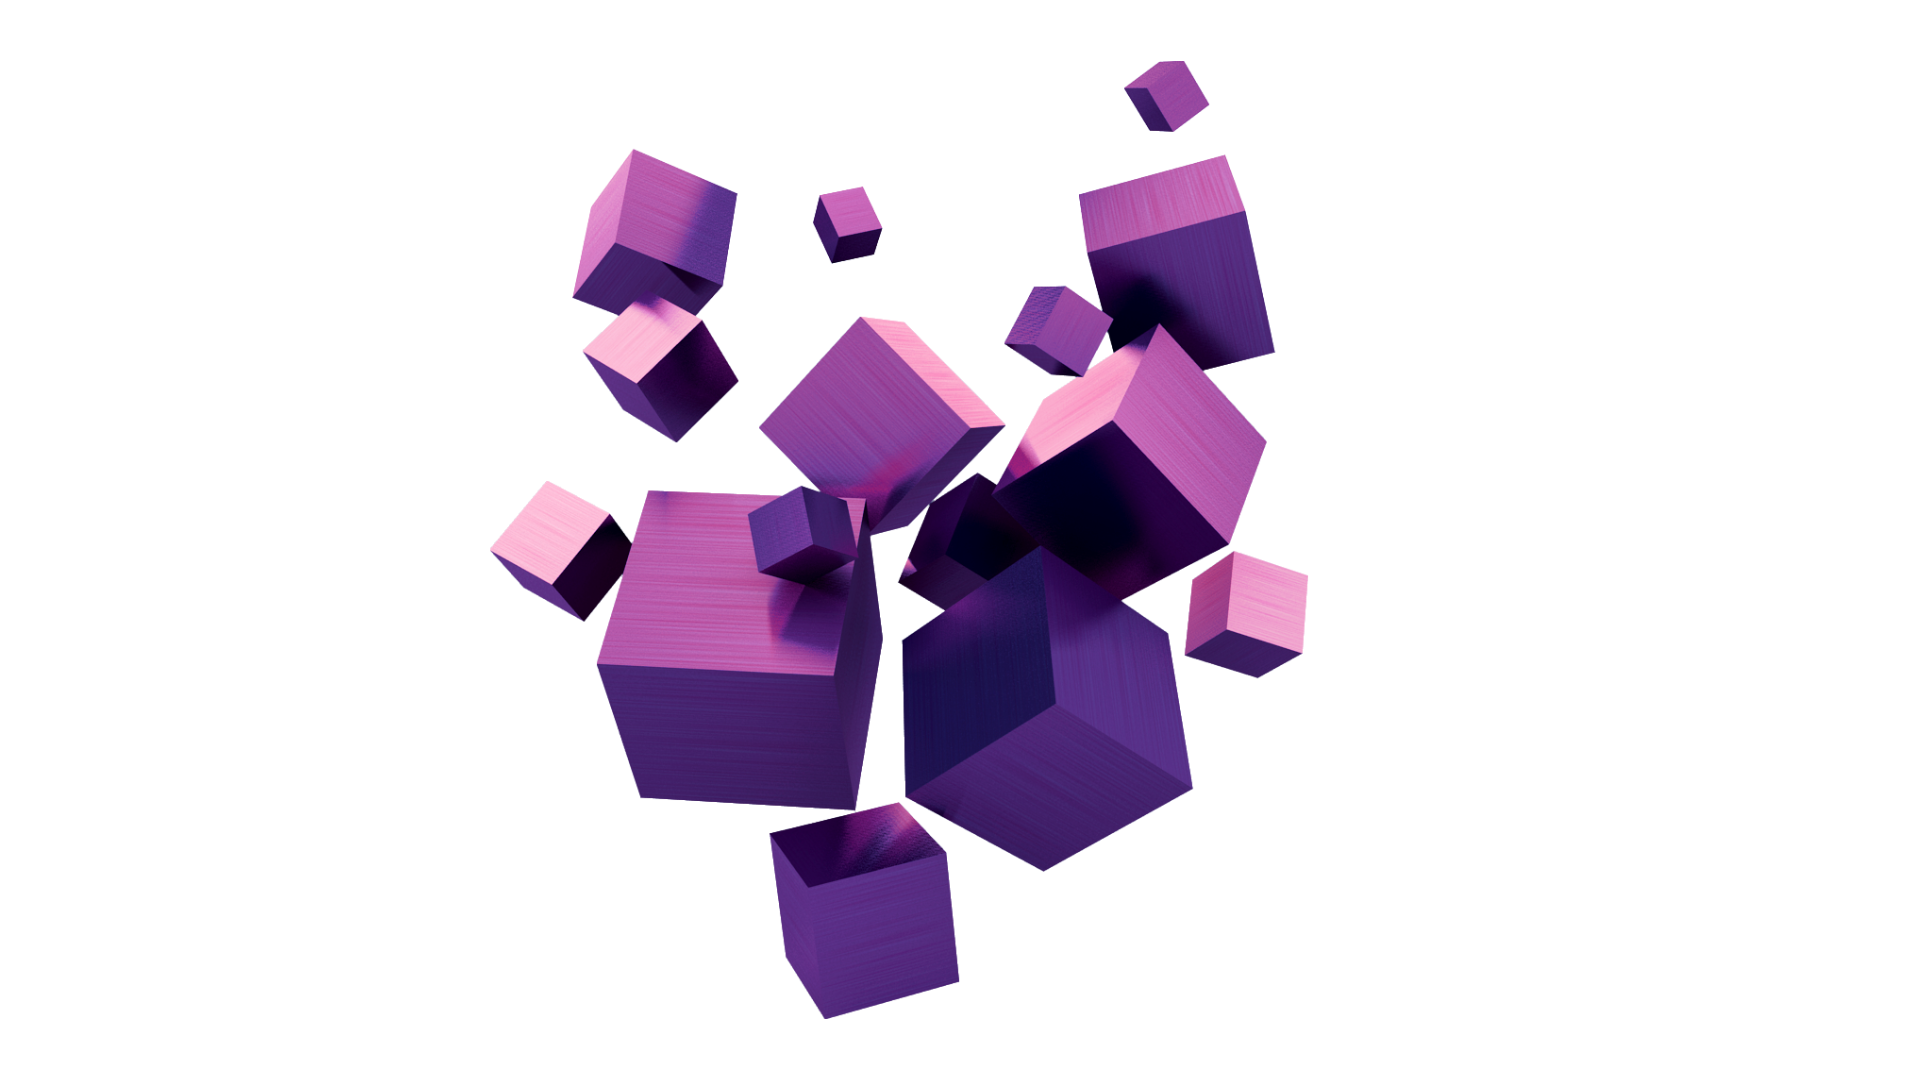
\includegraphics[width=\columnwidth]{13.png}
    \caption{Blocks}
    \label{Figure 2}
\end{figure}

\lipsum[5](see Figure~\ref{Figure 2,Figure 3})

\section*{Conclusion}
\; \; %% '\; \;' is required for indention
\lipsum[8]

\lipsum[8]

\lipsum[8]

\section*{Acknowledgments}
\; \; %% '\; \;' is required for indention
\lipsum[1]

\section*{Author Contributions}
\; \; %% '\; \;' is required for indention
The author did not receive any external help to write this paper/ The authors provided the following contributions: Author 1, Author 2 - Statistical Analysis, Author 3 - Data Visualization, etc.

%% Alphabetical References
%\bibliographystyle{unsrtnat}   %No abbreviation of First Name
\bibliographystyle{abbrvnat}    %Abbreviation of First Name
\bibliography{references} %% To edit the references copy paste the BibTex citation format in the references.bib file in the left

\section*{Appendices}
\lipsum[1]


\begin{figure}[H] %'[H]' forces the figure to stay in the relative position of the text it is located
    \centering
    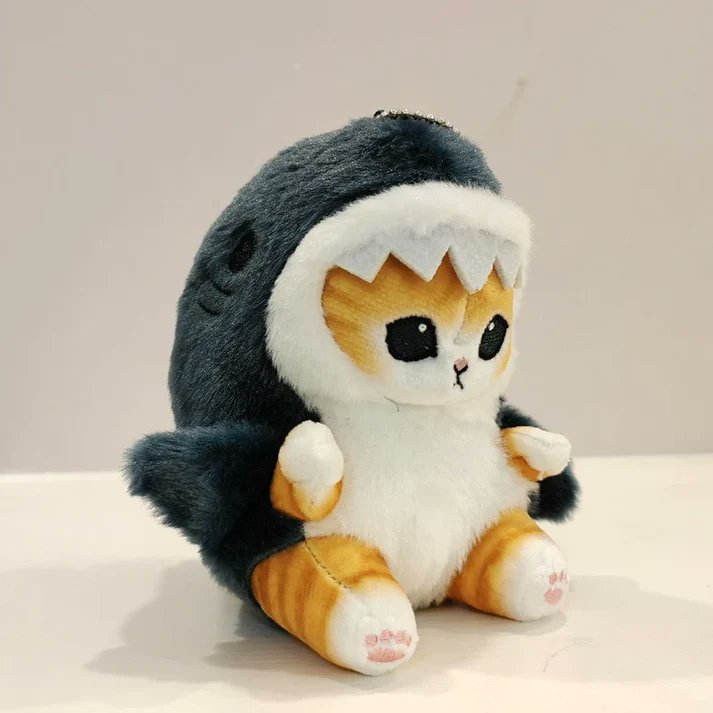
\includegraphics[width=\columnwidth]{catto.png}
    \caption{Scary Shark Catto}
    \label{Figure 3}
\end{figure}

    
\lipsum[1]

\subsection*{Appendix 1}

\lipsum[1]

\lipsum[1]

\lipsum[2]

\lipsum[2]

\lipsum[2]
\end{document}